\documentclass[fontsize=11bp]{beamer}
\useoutertheme{infolines}
\usepackage{graphicx} % Required for inserting images
\usepackage{caption}
\usepackage{subcaption}
\usepackage{hyperref}
\definecolor{Azul}{rgb}{0.1,0.1,0.6}
\title{Física estadística de las epidemias}
\subtitle{Código del TFG: FS22-13-FSC}
\author{Antonio Rivas Blanco}
\date{22 de Junio de 2023}
\mode<presentation>{\usetheme{Ilmenau}}%Ilmenau

\usepackage{pgfpages}
\setbeameroption{hide notes}%para tener notas del presentador. hide notes: solo muestra la presentación,
%show only notes: muestra solo las notas


\begin{document}
\renewcommand{\figurename}{ } %Cambiar el nombre de Figura
\frame{\titlepage 
        \begin{figure}[H]
        \centering
        
\includegraphics[scale=0.14]{logo_ciencias.png}
    \end{figure}
}

\begin{frame}
    \tableofcontents[sectionstyle=show,subsectionstyle=show/shaded/hide,subsubsectionstyle=show/shaded/hide]
\end{frame}

\section{Abstract}
\begin{frame}
\small Epidemics have had an impact of doubtless importance in recent times, so it is necessary to control the expansion of 
diseases for a prosperous development of society.

In this paper an introduction about different transmision models will be given. We will focus on the study of the 
simplest one, the susceptible-infected-susceptible model \textcolor{Azul}{(SIS)}. We will talk about the mathematical treatment for 
solving the model, which we will do by two methods: simulating compatible paths with the model using \textcolor{Azul}{Gillespie's algorithm} and solving numerically 
\textcolor{Azul}{Langevin equation}. To do this, we will use different algorithms programmed in \textcolor{Azul}{Python} language.

Finally, the simulations will be represented for differents values of the parametres which will allow us to draw conclusions 
about the system's stochastic behaviour and different control methods.\newline

\textbf{Keywords:} stochastic processes; phase transitions; master equation; Gillespie's algorithm; Fokker-Plank equation; Langevin's equation
\end{frame}

\section{Introducción}
\begin{frame}[t]{Impacto de las epidemias en la sociedad}
    \begin{figure}
        \centering
        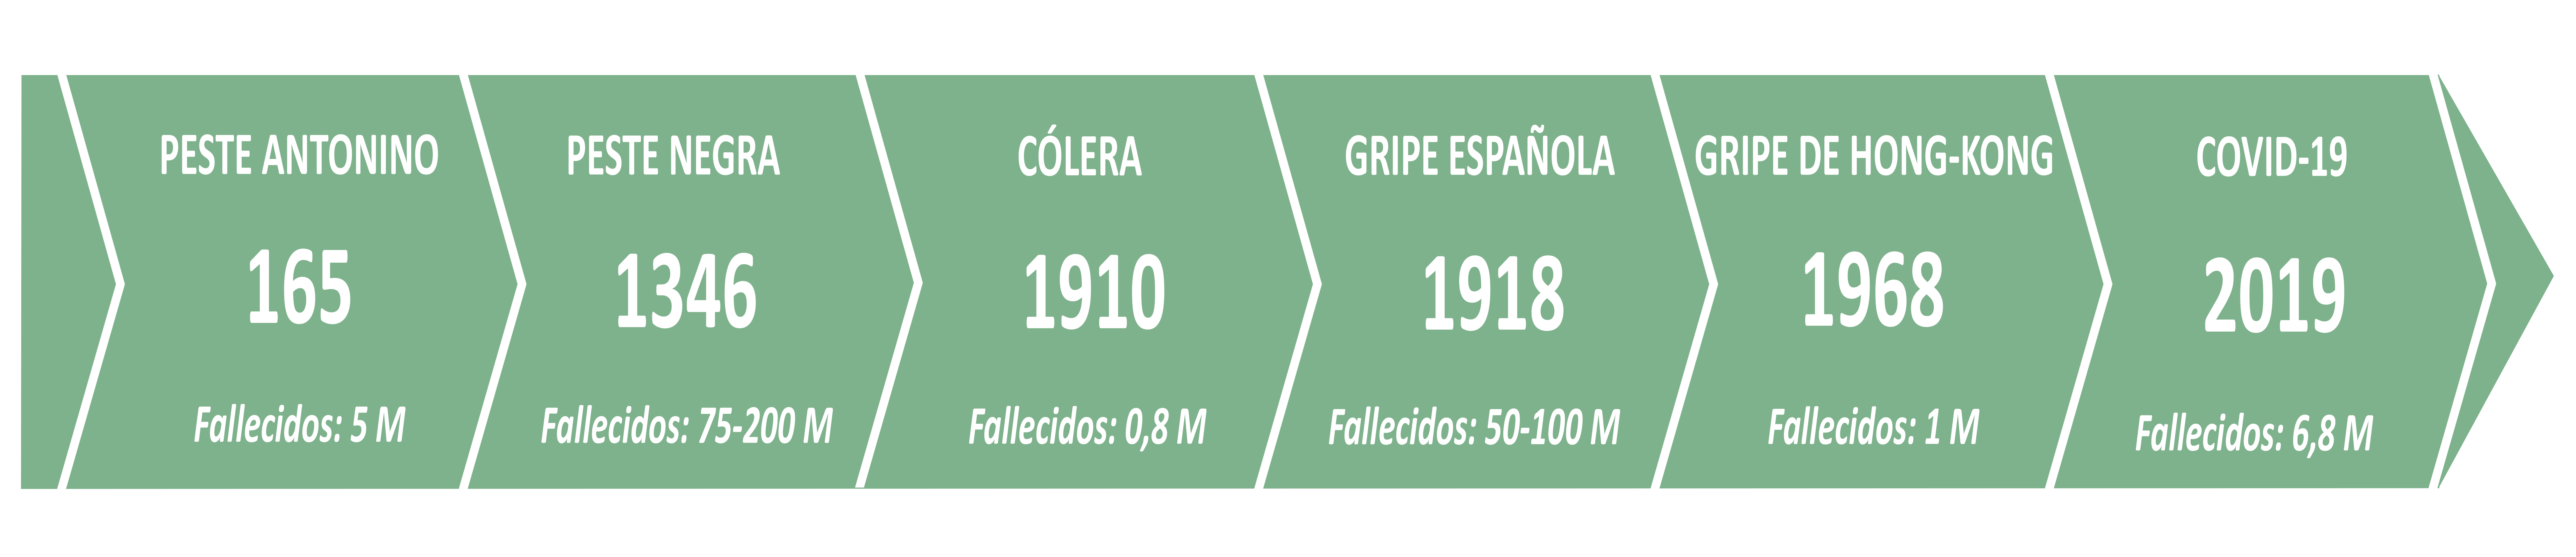
\includegraphics[width=0.75\textwidth]{Linea tiempo Antonio.png}
    \end{figure}
    \begin{block}{}
        \begin{itemize}[<+->]
            \item ¿A qué impactan las epidemias?
            \item ¿Por qué es necesario el estudio de estas?
            \item ¿Cómo podemos estudiarlas?
            
            \note<1>{Las epidemias tienen impacto además de en la salud pública, en la sociedad, economía, política...}
            \note<2>{Para entender cómo se transmiten, lo que nos permitirá tomar medidas para minimizar los efectos.}
            \note<3>{Nos ayudaremos diferentes modelos en función de como se comporte la epidemia y de la física estadística para poder pronosticar comportamientos de la enfermedad.}

        \end{itemize}
    \end{block}    
\end{frame}


\section{Objetivos}
\begin{frame}[t]{Objetivos}
    En este Trabajo Fin de Grado se han planteado los siguientes objetivos:
        \begin{itemize}[<+->]
            \item Estudiar el modelo susceptible-infectado-susceptible (SIS).
            \item Utilizar métodos Montecarlo, la ecuación de Langevin y el
            algoritmo de Gillespie para estudiar la evolución del sistema.            
            \item Implementación en Python.
            \item Visualizar y analizar los resultados obtenidos para distintos órdenes de población
            e interacción. En concreto, nos centraremos en el estudio del diagrama de fase.

            \note<1>{Estudiar modelo SIS, tamaño finito $\rightarrow$ fluctuaciones $\rightarrow$ Teoría procesos estocásticos}
            \note<2>{Métodos Montecarlo, ecuaciones (Lange, algoritmo Gillespie) para estudiar sistema}
            \note<3>{Python para resolver}
            \note<4>{Visualizar y analizar resultados, centrándonos diagrama de fase}
        \end{itemize}

\end{frame}


\section{Materiales y métodos}
\begin{frame}[t]{Generación de números aleatorios}
\note<1>{NÚMEROS ALEATORIOS: Son necesarios en los métodos Montecarlo, en concreto nosotros los usamos en el algoritmo de Gillespie y en la resolución de la ecuación de Langevin.\newline}
\only<2-4>{\begin{block}{Generadores de números (pseudo)aleatorios}
        \textbf{Uniformes:} Generador lineal congruencial\newline
        \textbf{No uniformes:} Método transformada inversa
        \note<2>{GENERADORES DE NÚMEROS ALEATORIOS UNIFORMES: Son algoritmos que nos permiten obtener una secuencia de números determinista y periódica cuyas propiedades son muy parecidas a una secuencia totalmente aleatoria.\newline Están incluidos en bibliotecas de Python, pero conviene saber como funcionan.}
        \note<2>{\newline$n_0$ semilla, $a$ multiplicador, $b$ incremento, $M$ Cota superior\newline Son muy sensibles a los parámetros, como se ve en la figura}
\end{block}}
\only<3>{ \begin{figure}[H]
        \begin{subfigure}[b]{0.4\textwidth}
          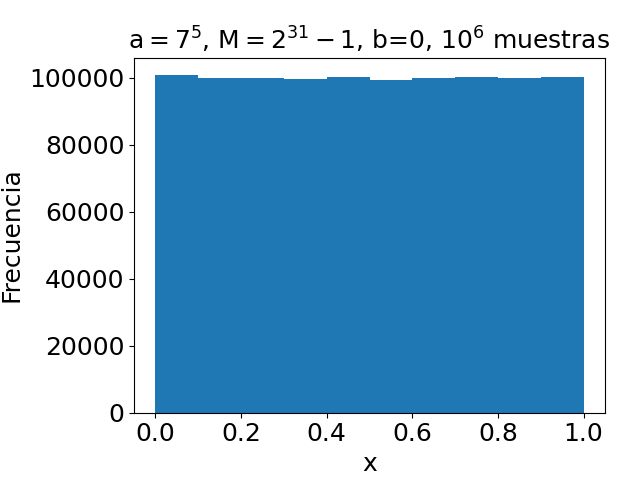
\includegraphics[width=\textwidth]{lgc bueno.png}
          \label{fig:buenos parámetros}
        \end{subfigure}
        \begin{subfigure}[b]{0.4\textwidth}
          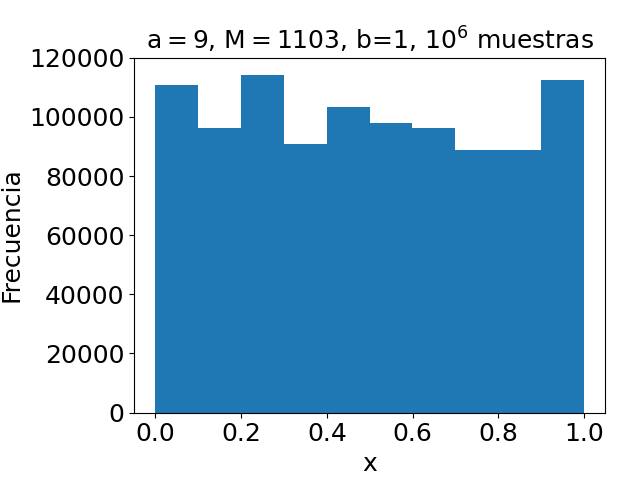
\includegraphics[width=\textwidth]{lgc malo.png}
          \label{fig:malos parámetros}
        \end{subfigure}
      \end{figure}}
\only<4>{\begin{figure}[H]
    \centering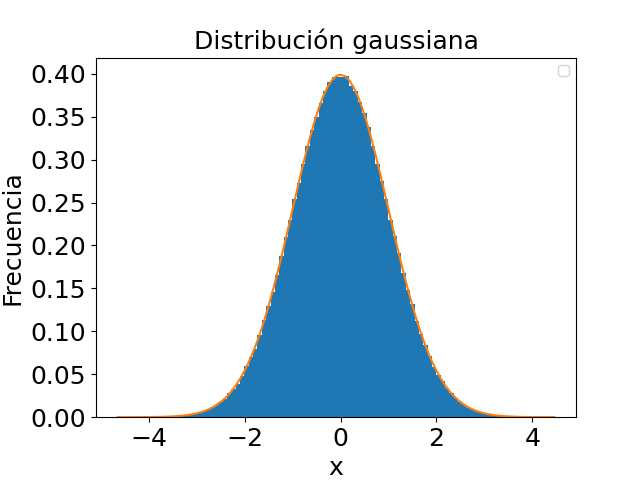
\includegraphics[width=0.45\textwidth]{gauss.png}
  \end{figure}}


\end{frame}
\begin{frame}[t]{Entorno de programación}
\note<1>{Se ha utilizado Python para las simulaciones, instalado en Visual Studio Code, donde también se ha realizado la memoria y la presentación\newline}    
\only<2>{    \begin{block}{Bibliotecas}
        \begin{itemize}
            \item Numpy
            \item Matplotlib
            \note<2>{Nos proporciona una gran cantidad de funciones matemáticas y cálculo más eficiente al de Python}
            \note<2>{\newline Permite graficar para un estudio más visual de los resultados}
        \end{itemize}
    \end{block}
    \onslide<2>{\begin{columns}[onlytextwidth]
        \begin{column}{.45\textwidth}
        \begin{figure}
          
\includegraphics[width=0.5\textwidth]{numpy.png}
          \caption*{\tiny{\url{https://numpy.org/}}}
        \end{figure}
        \end{column}
        \hfill
        \begin{column}{.45\textwidth}
        \begin{figure}
          
\includegraphics[width=0.85\textwidth]{matplotlib.png}
          \caption*{\tiny{\url{https://pypi.org/project/matplotlib/}}}
        \end{figure}
        \end{column}
        \end{columns}
    }
}
\end{frame}

\begin{frame}[t]{Modelo SIS: características}
    \note<1>{Blanco}
 \only<2>{\begin{figure}
                \centering 
                \includegraphics[width=\textwidth]{Antonio Arregalao.png}
           \end{figure}}
            \note<2>{ Definir $n_i$, $n_s$, $N=$cte e interacción homogénea}
\end{frame}

\begin{frame}[t]{Procesos estocásticos}
\note<1>{$n_i$ es una variable estocástica, evoluciona de manera no determinista. Concretamente es un proceso de Markov, la evolución depende solo del estado en el que se encuentra el sistema}    
\only<2-5>{\begin{block}{Ecuación maestra}
          \begin{itemize}
            \item <3-> Estado del sistema: $\vec{n}(t)= \left[ n_i(t),n_s(t) \right]\Longrightarrow$$P(\vec{n},t|\vec{n}_0,t_0)$.
          \end{itemize}  
          \onslide<4->{$$\dfrac{\partial P(\vec{n},t)}{\partial t}=\sum_{\vec{n}^{\prime}}\left[ W(\vec{n}^{\prime}\rightarrow\vec{n}) P(\vec{n}^{\prime},t) - W(\vec{n}\rightarrow\vec{n}^{\prime}) P( \vec{n},t)\right]$$}
    \note<2>{Ecuación diferencial $\rightarrow$ determinista, que describe evolución probabilidad de proceso de
Markov en sistemas cambian de estado de manera continua. Útil para procesos con nº estados discreto (Ya que
tendremos un sistema de ecs de orden del nº de estados).}
\note<4>{Probabilidad de encontrar en el estado $\vec{n}$ en el instante $t$ dadas unas condiciones iniciales.}
\end{block}
\only<5>{
    \begin{columns}
        \begin{column}{0.5\textwidth}
            \onslide<5>{\begin{figure}
                \centering
                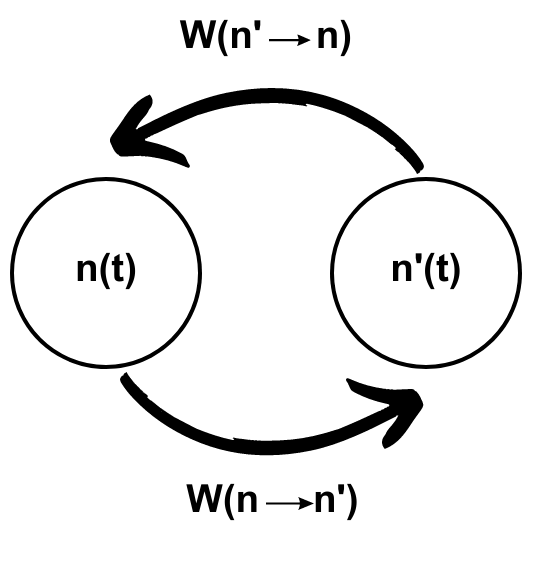
\includegraphics[scale=0.225]{n.png}
            \end{figure}}
        \end{column}
         
        \begin{column}{0.45\textwidth}
            \begin{block}{\small{Tasas del modelo SIS}}
                \onslide<5>{\small{$$W_+\equiv W(n\rightarrow n+1)=\lambda n\left( 1-\dfrac{n}{N} \right)$$
                $$W_-\equiv W(n\rightarrow n-1)=\mu n$$}}
            \end{block}
        \end{column}
    \end{columns}
    }
    }
\note<5>{Es una ecuación de continuidad de la probabilidad, la que entra menos lo que sale.}

\only<6-12>{
    \only<6->{\begin{block}{Algoritmo de Gillespie}
        \begin{itemize}
            \item<6-> $P(\vec{n},t|\vec{n}_0,t_0)\; \rightarrow \; P(j,\tau|\vec{n},t)$
            \item<7-> ¿Cuándo? $\tau \sim exp(\textup{media}=W_0)\qquad$ con $W_0=\sum_{j}W_j$ 
            \item<8-> ¿Qué? $P(j)=W_j/W_0$
        \end{itemize}
        \note<8>{$j$ es el entero más pequeño tal que $\sum_{j^\prime=1}^{j}W_{j^\prime}>r_2W_0$
        \newline con $r_2\in [0,1]$\newline $\tau$ lo obtenemos con transformada inversa también y $r_1\in[0,1]$}
        \begin{enumerate}
            \item<9-> Condiciones iniciales: $t=t_0$, $\vec{n}=\vec{n}_0$.
            \item<10-> $W_j(\vec{n})\;\rightarrow\;W_0(\vec{n})$
            \item<11-> Calculamos $\tau$ y $j$.
            \item<12-> Actualizamos el sistema y repetimos desde el paso 2.
    \end{enumerate}
\end{block}}
        

}
\only<13>{\begin{figure}
    \centering
    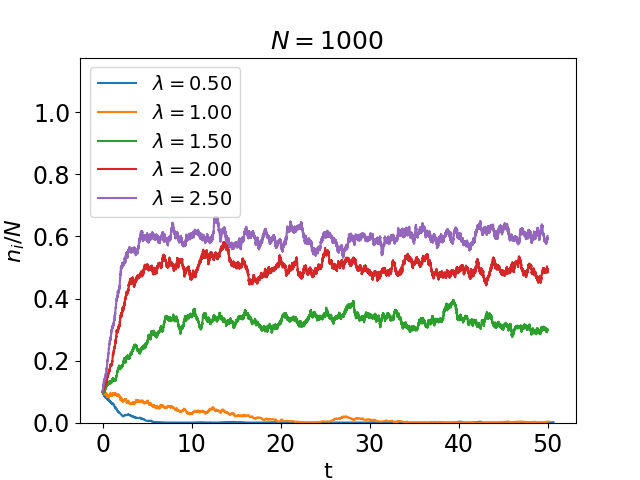
\includegraphics[scale=0.45]{ni_t_1000.png}
\end{figure}
}


\only<14-17>{\begin{block}{Ecuación de Fokker-Planck}
    \note<19>{desarrollo en serie a 2º orden de la ecuación Maestra $\rightarrow$ ecuación determinista para la probabilidad, pero en
    este caso de una variable cuasicontinua. Es algo más fácil de resolver que la ecuación maestra}
\only<14>{\onslide<14>{Nueva variable: $x=n_i/N$}}  
\only<15>{\onslide<15>{
    \begin{equation*}
        \begin{split}
            \partial_t \tilde{P}(x,t)&=-\partial_x[ \overbrace{\left( \lambda x (1-x)-\mu x\right)}^{A(x)}\tilde{P}(x,t)]\\
            &+\dfrac{1}{2}\partial_x^2[\underbrace{\dfrac{1}{N}\left( \lambda x (1-x)+\mu x\right)}_{B(x)}\tilde{P}(x,t) ]+\mathcal{O} (N^{-2})+\ldots
        \end{split}
        \end{equation*}}
}

\only<16>{\onslide<16>{\begin{equation*}
    \begin{split}
        \partial_t \tilde{P}(x,t)&=-\partial_x[ \overbrace{\left( \lambda x (1-x)-\mu x\right)}^{A(x)}\tilde{P}(x,t)]\\
        &+\dfrac{1}{2}\partial_x^2[\underbrace{\dfrac{1}{N}\left( \lambda x (1-x)+\mu x\right)}_{B(x)}\tilde{P}(x,t) ]+\mathcal{O} (N^{-2})+\ldots
    \end{split}
    \end{equation*}
\begin{equation*}
    \partial_tP(x,t)=-\partial_x\left[ A(x)P(x) \right]+\frac{1}{2}\partial_x^2\left[ B(x)P(x) \right]
\end{equation*}}}

\only<17>{\small{\onslide<17>{\begin{equation*}
    \begin{split}
        \partial_t \tilde{P}(x,t)&=-\partial_x[ \overbrace{\left( \lambda x (1-x)-\mu x\right)}^{A(x)}\tilde{P}(x,t)]\\
        &+\dfrac{1}{2}\partial_x^2[\underbrace{\dfrac{1}{N}\left( \lambda x (1-x)+\mu x\right)}_{B(x)}\tilde{P}(x,t) ]+\mathcal{O} (N^{-2})+\ldots
    \end{split}
    \end{equation*}
\begin{equation*}
    \partial_tP(x,t)=-\partial_x\left[ A(x)P(x) \right]+\frac{1}{2}\partial_x^2\left[ B(x)P(x) \right]
\end{equation*}
\begin{equation*}
    \dot{x}=A(x)+\sqrt{B(x)}\;\xi(t)
\end{equation*}
}
}
}
\end{block}

}

\only<18-20>{\begin{block}<18-20>{Ecuación de Langevin}
    \onslide<18->{Para nuestro sistema queda:\newline
    $$\dot{x}=\lambda x (1-x)-\mu x+\dfrac{1}{\sqrt{N}}\sqrt{\lambda x (1-x)+\mu x} \; \xi(t)$$}
    \end{block}
    \onslide<19->{Si tomamos $N\to \infty$, el estado estacionario será:}
    \onslide<20>{\begin{columns}
        \begin{column}{0.5\textwidth}
            \onslide<20>{$$x^{est}=\left\{ \begin{array}{lr} 0 & si \lambda < \mu\\ 1-\dfrac{\mu}{\lambda} & si \lambda \ge \mu \end{array} \right.$$
            }
        \end{column}
         
        \begin{column}{0.5\textwidth}
            \onslide<20>{\begin{figure}
                
                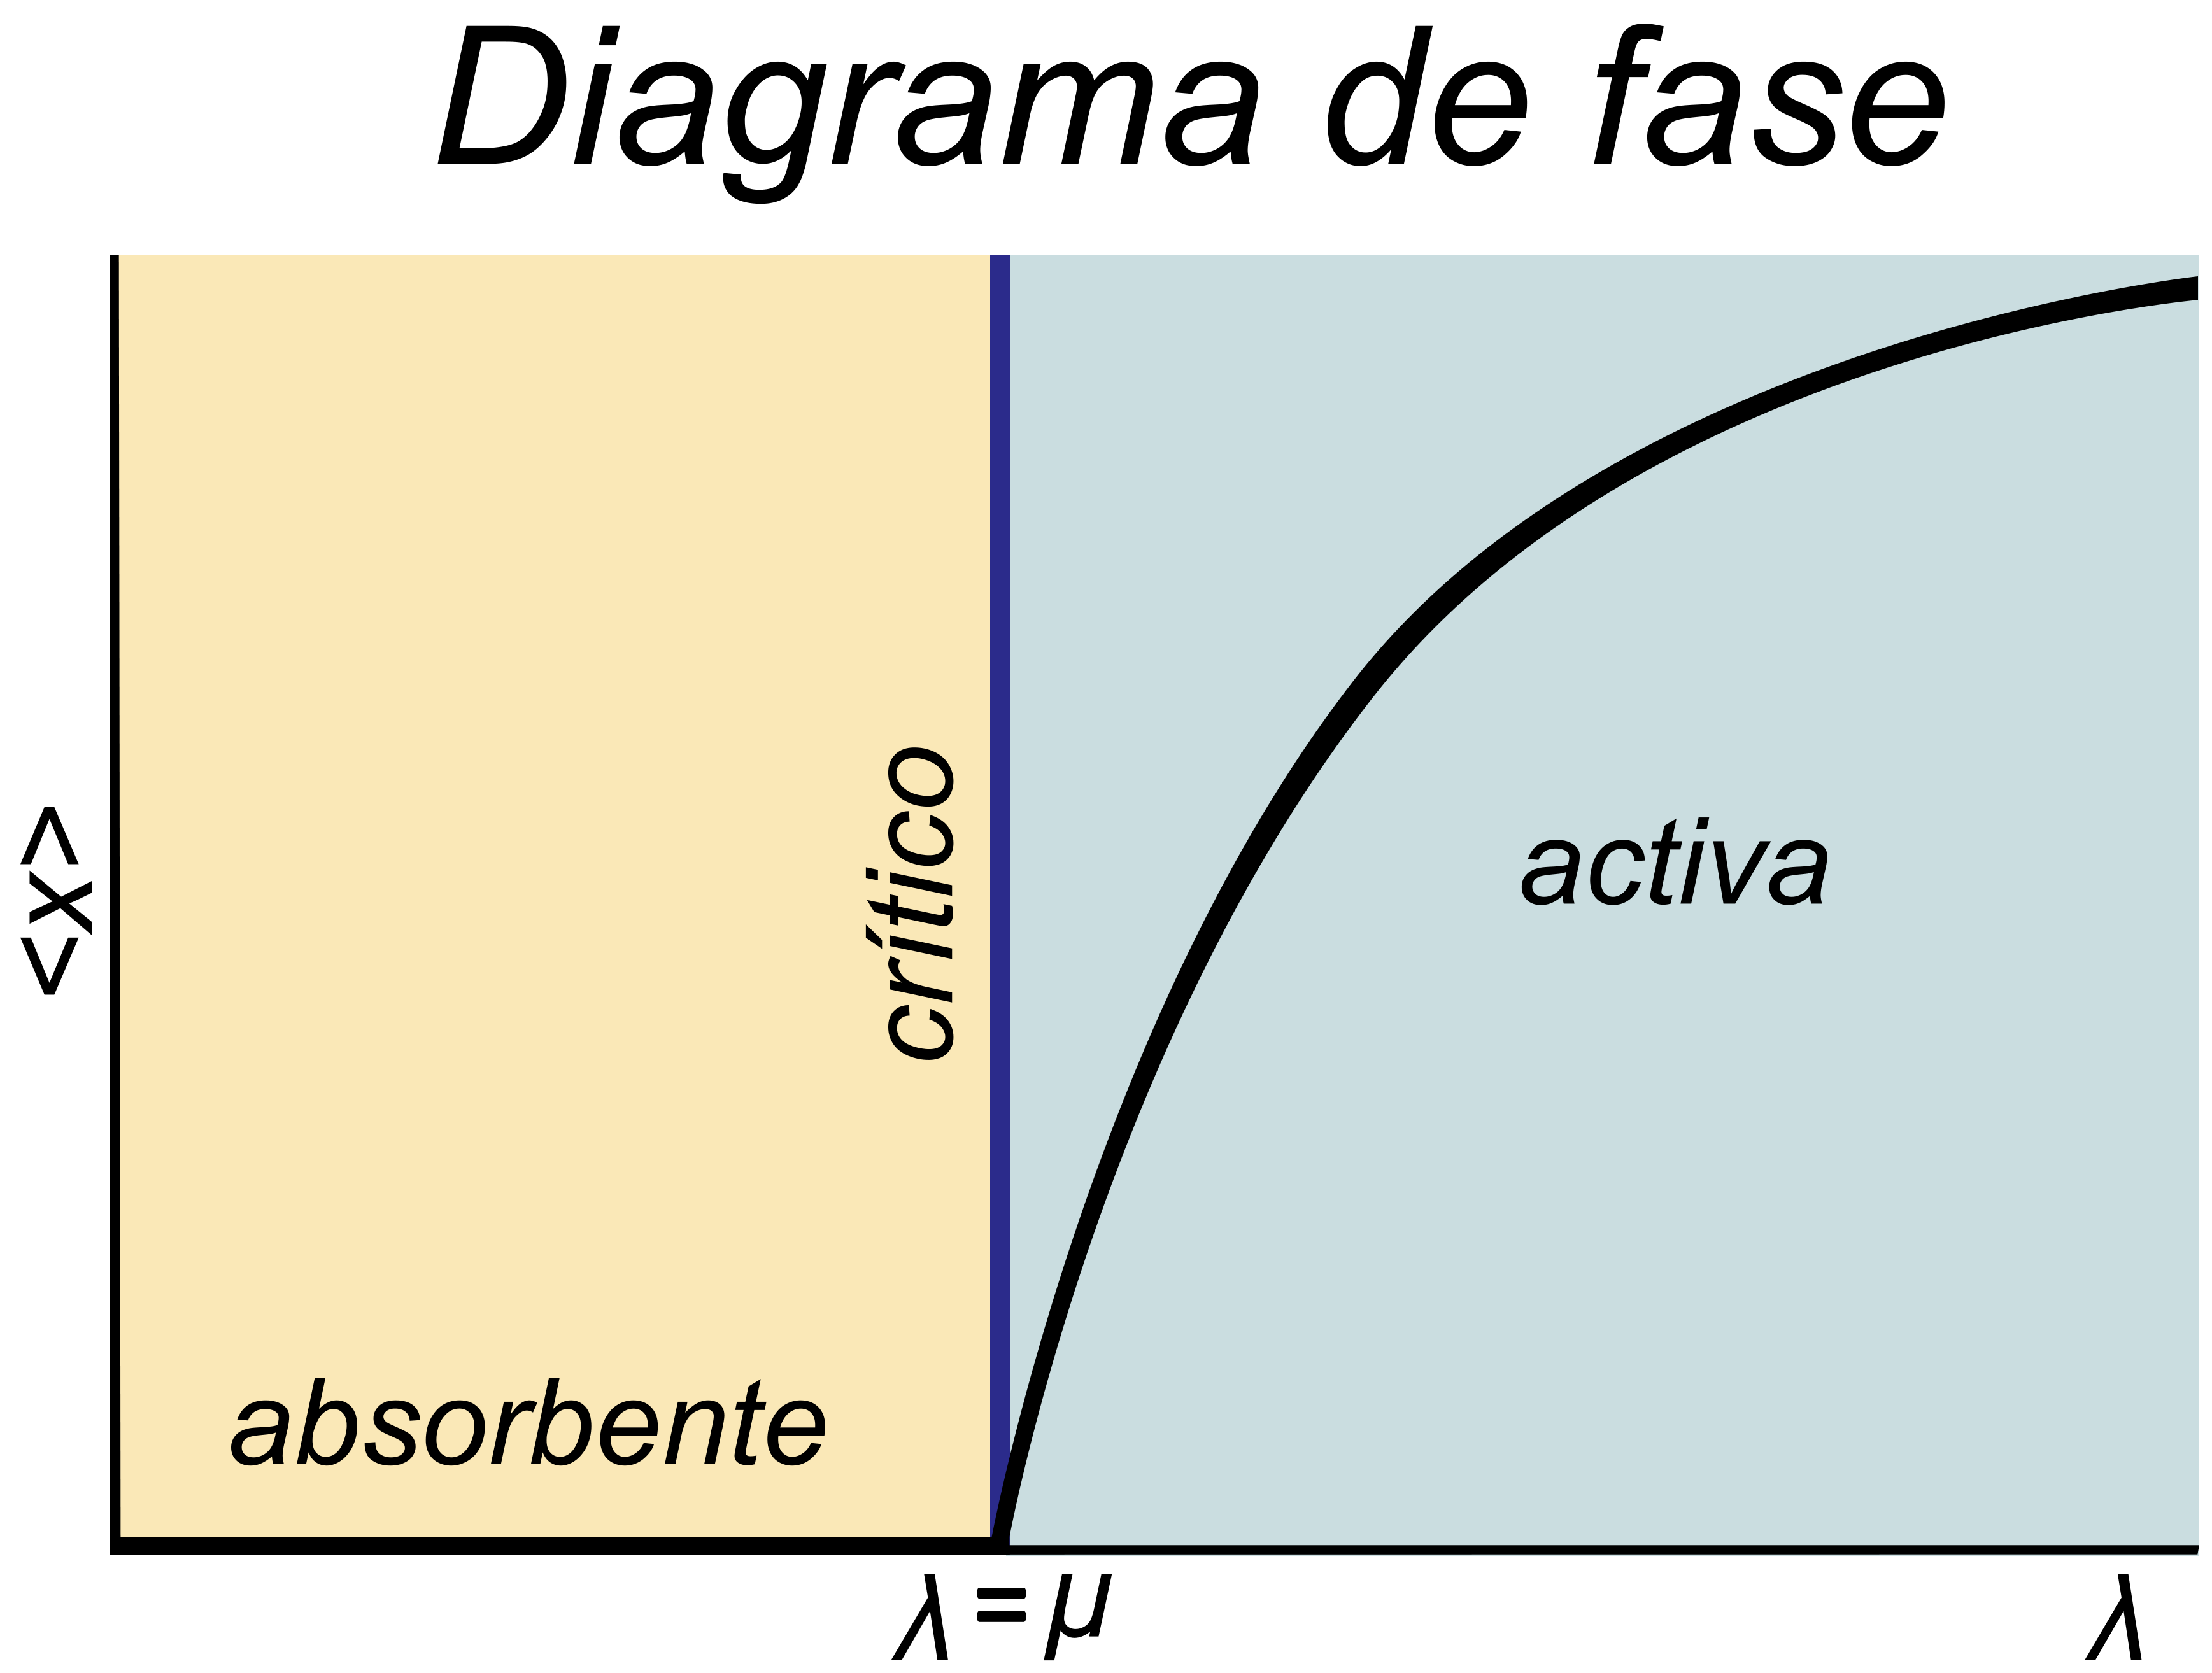
\includegraphics[width=0.5\textwidth]{Antonio Arreglao 2.png}
            \end{figure}}
        \end{column}
    \end{columns}

    }
     
}

\end{frame}

\section{Resultados}
\begin{frame}[t]{Resultados}
\note<1>{Se estudiaran series temporales, condiciones iniciales, diagrama de fase y desviación estándar(amplitud fluctuaciones). Tomaremos 
$\mu=1$ y condición iniciales $N/10$ para todos los casos.\newline
Las dimensiones $\mu$ y de $\lambda$ son de $tiempo^{-1}$. Utilizamos sistema de unidades arbitrario,
lo que quiere decir que se producirá una recuperación por hora, día, mes... Debido a esta arbitrariedad en las unidades,
hemos decidido omitirlas en todas las gráficas.
}
\only<2>{\begin{block}<2>{Series temporales}
    \onslide<2>{\begin{figure}[H]
        \begin{subfigure}[b]{0.45\textwidth}
          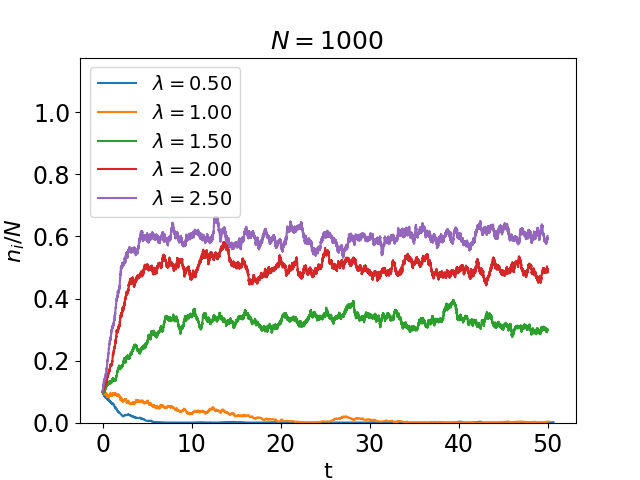
\includegraphics[width=\textwidth]{ni_t_1000.png}
          \caption{Gillespie}
          \label{fig:n vs t 1000}
        \end{subfigure}
        \begin{subfigure}[b]{0.45\textwidth}
          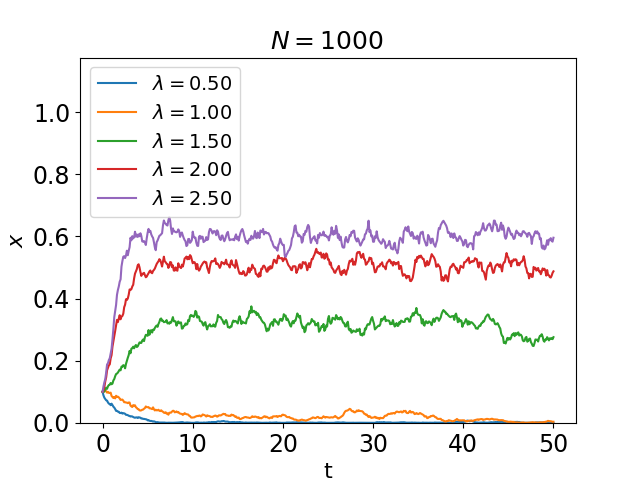
\includegraphics[width=\textwidth]{x vs t fockerplanck.png}
          \caption{Langevin}
          \label{fig:x vs t 1000}
        \end{subfigure}
      \end{figure}
    }
\end{block}
\note<3>{Como se comprueba, las fluctuaciones son menores en este caso}
}


    \only<3>{\begin{block}<3>{Series temporales}
        \onslide<3>{\begin{figure}[H]
            \begin{subfigure}[b]{0.45\textwidth}
              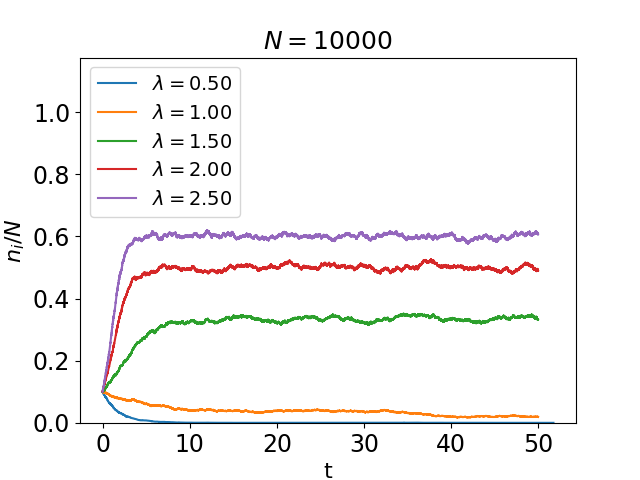
\includegraphics[width=\textwidth]{ni_t_10000.png}
              \caption{Gillespie}
              \label{fig:n vs t 10000}
            \end{subfigure}
            \begin{subfigure}[b]{0.45\textwidth}
              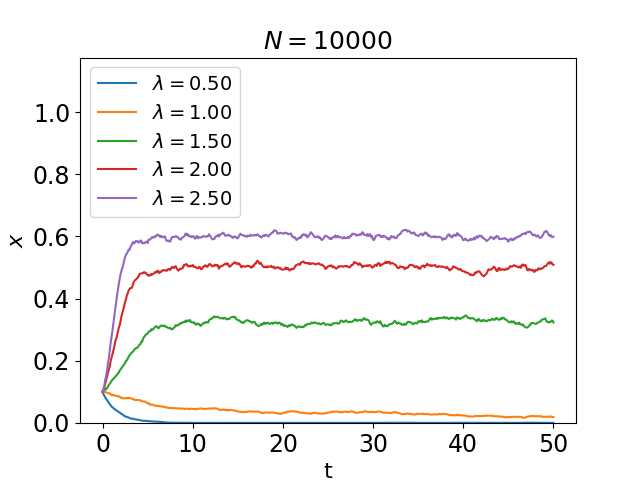
\includegraphics[width=\textwidth]{x vs t fockerplanck 10000.png}
              \caption{Langevin}
              \label{fig:x vs t 10000}
            \end{subfigure}
          \end{figure}
        }
    \end{block}
    \note<3>{Como se comprueba, las fluctuaciones son menores en este caso}
}

\only<4>{    \begin{block}<4>{Condiciones iniciales}
    \onslide<4>{\begin{figure}[H]
        \begin{subfigure}[b]{0.45\textwidth}
          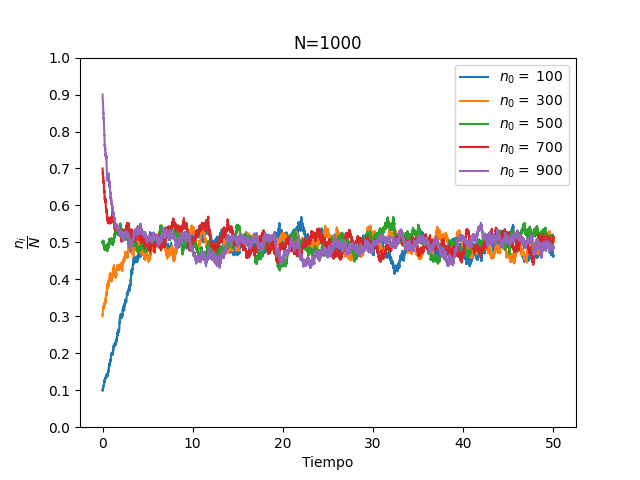
\includegraphics[width=\textwidth]{Ccii.png}
          \caption{Gillespie}
          \label{fig:ccii gillespie}
        \end{subfigure}
        \begin{subfigure}[b]{0.45\textwidth}
          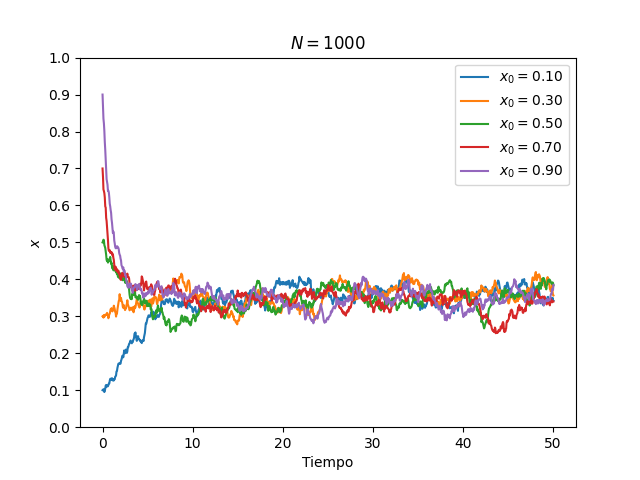
\includegraphics[width=\textwidth]{cciifockerplanck.png}
          \caption{Langevin}
          \label{fig:ccii langevin}
        \end{subfigure}
      \end{figure}}
\end{block}
\note<4>{Como se ha visto el estado estacionario no depende de las condiciones iniciales, solo de las tasas de recuperación
tal y como aparece en las figuras}
}

\only<5>{\begin{block}<5>{Diagrama de fase}   
    \onslide<5>{\begin{figure}[H]
        \begin{subfigure}[b]{0.45\textwidth}
          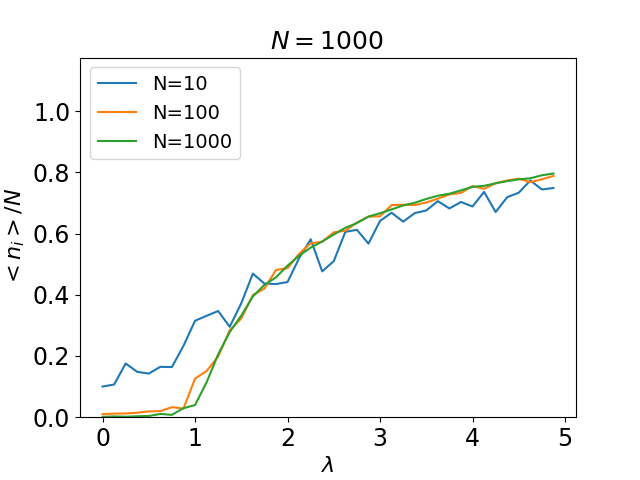
\includegraphics[width=\textwidth]{40 puntos 10_100_1000.png}
          \caption{Gillespie}
          \label{fig:fase gillespie}
        \end{subfigure}
        \begin{subfigure}[b]{0.45\textwidth}
          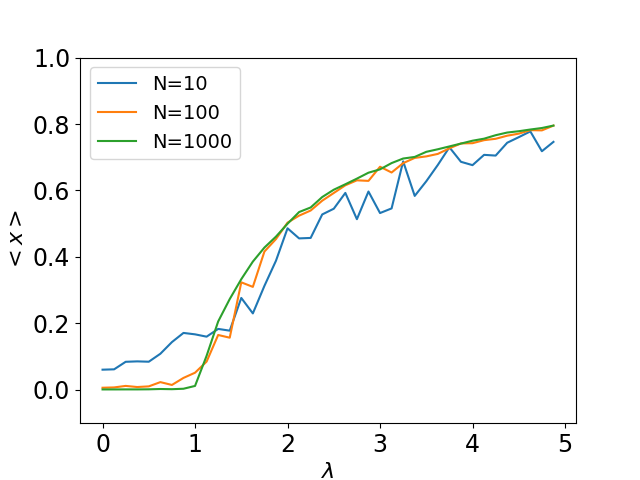
\includegraphics[width=\textwidth]{xmedia vs lambda focker.png}
          \caption{Langevin}
          \label{fig:fase langevin}
        \end{subfigure}
      \end{figure}}
\end{block}
\note<5>{Se ajustan bastante bien al diagrama esperado, si bien en el caso en el que la población es de $10$ individuos
esta curva es levemente distinta, ya que el cambio de estado de un individuo cambia el $10\%$ del sistema. A esto tenemos que 
sumarle que nuestra condición inicial para esta población es que un individuo está infectado, por lo que las propias fluctuaciones llevan 
a la extinción de infectados y nuestra simulación añade uno infectado para seguir ejecutándose, lo que provoca que el número medio de infectados
sea no nulo en la zona absorbente.}
}

\only<6>{    \begin{block}<6>{Desviación estándar}
    \onslide<6>{\begin{figure}[H]
        \begin{subfigure}[b]{0.45\textwidth}
          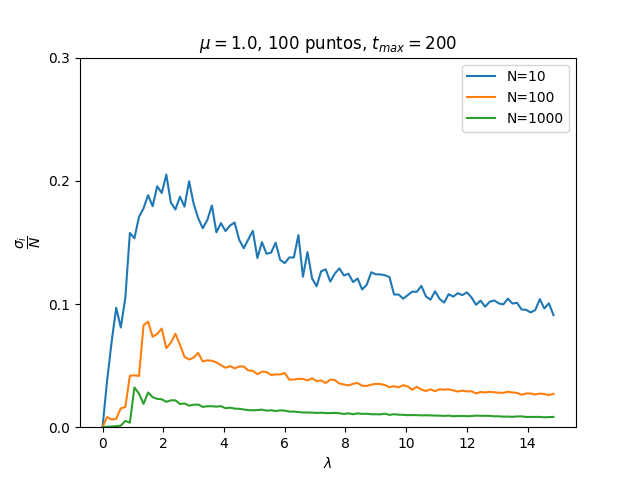
\includegraphics[width=\textwidth]{sigma_lambda.png}
          \caption{Gillespie}
          \label{fig:sigma gillespie}
        \end{subfigure}
        \begin{subfigure}[b]{0.45\textwidth}
          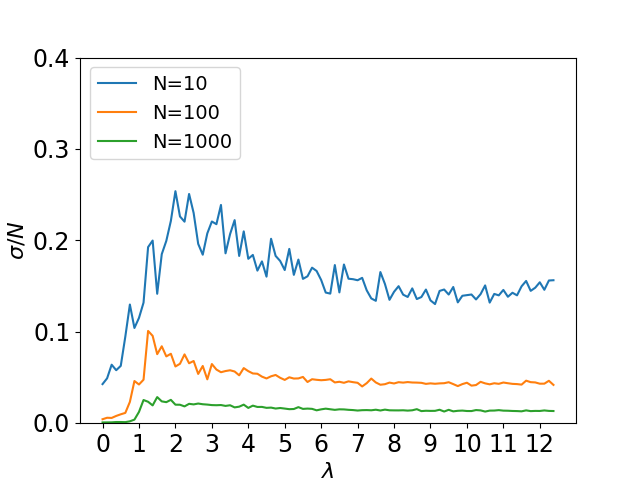
\includegraphics[width=\textwidth]{sigmalambdafocker.png}
          \caption{Langevin}
          \label{fig:sigma langevin}
        \end{subfigure}
      \end{figure}}
\end{block}
\note<6>{Como se comprueba, comportamiento similar. Estas fluctuaciones son mayores en el entorno del punto crítico, 
tal y como esperabamos. Langevin $N=10$ una pequeña sobreestimación de la desviación estándarya que la aproximación
de Fokker-Planck no se cumple. Podemos utilizar esta desviación estándar como las barras de error,
pero hemos decidido no incluirlas en el diagrama de fase para no sobrecargar la imagen.}
}


\end{frame}


\section{Conclusions}
\begin{frame}[t]{Conclusions}
    \begin{itemize}[<+->]
        \item A brief introduction to stochastic processes has been conducted.
        \item We can use physics in other branches of knowledge.
        \item The use of mathematical models has allowed us to characterize the behaviour of epidemics.
        \item Programming is essential.
        \item We have examined the different phases of epidemics in our model and the effect of changing various parameters.
        \item Gillespie or Langevin?
        \end{itemize}

        \note<3>{Such as epidemiology, sociology or biology.}
        \note<4>{because when we consider non-ideal situations, the majority of problems don't have analytical solution.}
\note<6>{On one hand, with the Gillespie algorithm, we do not make any approximations, so the results obtained will be good for any 
value of the different parameters in our system. One drawback of this method is the computational time. It increases with population and
infection rate.\newline

On the other hand, in the case of the Langevin equation, we have the restriction that we need a large population to apply 
the approximation. But with pur types of systems, we can apply it. The main advantage of this method is the 
simulation time, which is practically fixed since we choose the time step for the resolution of the differential equation. 
.\newline In general, as mentioned, both methods are good but it is better to use the Langevin equation due to the shorter simulation time.}
\end{frame}
\section*{Bibliografía}
\begin{frame}{Bibliografía}
    \begin{enumerate}
        \item Gerardo Chowell et al. ''Mathematical models to characterize early epidemic
        growth: A review". En: \textit{Physics of life reviews 18} (2016), págs. 66-97.
        \item Romualdo Pastor-Satorras et al. ''Epidemic processes in complex networks". En:\textit{
        Reviews of modern physics} 87.3 (2015), pág. 925.
        \item Daniel T Gillespie. ''Stochastic simulation of chemical kinetics". En: \textit{Annu. Rev.
        Phys. Chem.} 58 (2007), págs. 35-55.
        \item Alan J McKane. \textit{Stochastic Processes.} 2009.
        \item Raúl Toral y Pere Colet. \textit{Stochastic numerical methods: an introduction for students and scientists.} John Wiley $\&$ Sons, 2014.
    \end{enumerate}
\end{frame}


\frame  {\titlepage 
        \begin{figure}[H]
        \centering
        
\includegraphics[scale=0.14]{logo_ciencias.png}
    \end{figure}
}

\begin{frame}
    \only<1>{\begin{block}{Ecuación maestra del modelo SIS}
        \onslide<1>{
        \begin{equation*}
            \begin{split}
                \partial_t P(n,t)&=W_+(n-1)P(n-1,t)+W_-(n+1)P(n+1,t)-\\
                &-W_-(n)P(n,t)-W_+(n)P(n,t)  
            \end{split}
            \label{eq:Ecuación maestra SIS}
        \end{equation*}\note<1>{Sistema de ecuaciones diferenciales acopladas, una cada estado. Generalmente no tiene solución analítica y tiene gran costo computacional resolverlo $\rightarrow$ Gillespie trayectorias (de la variable $n_i$) compatibles con la solución de
        esta ecuación.}
        }
        \end{block}
        \onslide<1>{\begin{figure}\centering 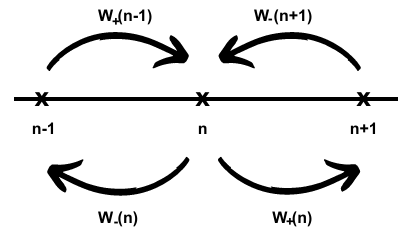
\includegraphics[scale=0.5]{ec maestra.png}\end{figure}}
    }

    \only<2>{\begin{block}<2>{Resolución de la ecuación de Langevin}
        \onslide<2>$$x(t+\Delta t)=x(t)+\overbrace{\Delta t\: A(x(t))}^{\textup{Euler}}+\underbrace{\sqrt{B(x(t))}\mathcal{G}(0,\sqrt{\Delta t})}_{\textup{Itô}}$$
    \end{block}}

    \only<3>{\begin{figure}
        \centering
        \includegraphics[width=\textwidth]{Tfg ANTONIO- 2 - fONDO EL otro.png}
    \end{figure}
        }
\end{frame}

\end{document}